% Options for packages loaded elsewhere
\PassOptionsToPackage{unicode}{hyperref}
\PassOptionsToPackage{hyphens}{url}
%
\documentclass[
]{article}
\usepackage{amsmath,amssymb}
\usepackage{iftex}
\ifPDFTeX
  \usepackage[T1]{fontenc}
  \usepackage[utf8]{inputenc}
  \usepackage{textcomp} % provide euro and other symbols
\else % if luatex or xetex
  \usepackage{unicode-math} % this also loads fontspec
  \defaultfontfeatures{Scale=MatchLowercase}
  \defaultfontfeatures[\rmfamily]{Ligatures=TeX,Scale=1}
\fi
\usepackage{lmodern}
\ifPDFTeX\else
  % xetex/luatex font selection
\fi
% Use upquote if available, for straight quotes in verbatim environments
\IfFileExists{upquote.sty}{\usepackage{upquote}}{}
\IfFileExists{microtype.sty}{% use microtype if available
  \usepackage[]{microtype}
  \UseMicrotypeSet[protrusion]{basicmath} % disable protrusion for tt fonts
}{}
\makeatletter
\@ifundefined{KOMAClassName}{% if non-KOMA class
  \IfFileExists{parskip.sty}{%
    \usepackage{parskip}
  }{% else
    \setlength{\parindent}{0pt}
    \setlength{\parskip}{6pt plus 2pt minus 1pt}}
}{% if KOMA class
  \KOMAoptions{parskip=half}}
\makeatother
\usepackage{xcolor}
\usepackage[margin=1in]{geometry}
\usepackage{color}
\usepackage{fancyvrb}
\newcommand{\VerbBar}{|}
\newcommand{\VERB}{\Verb[commandchars=\\\{\}]}
\DefineVerbatimEnvironment{Highlighting}{Verbatim}{commandchars=\\\{\}}
% Add ',fontsize=\small' for more characters per line
\usepackage{framed}
\definecolor{shadecolor}{RGB}{248,248,248}
\newenvironment{Shaded}{\begin{snugshade}}{\end{snugshade}}
\newcommand{\AlertTok}[1]{\textcolor[rgb]{0.94,0.16,0.16}{#1}}
\newcommand{\AnnotationTok}[1]{\textcolor[rgb]{0.56,0.35,0.01}{\textbf{\textit{#1}}}}
\newcommand{\AttributeTok}[1]{\textcolor[rgb]{0.13,0.29,0.53}{#1}}
\newcommand{\BaseNTok}[1]{\textcolor[rgb]{0.00,0.00,0.81}{#1}}
\newcommand{\BuiltInTok}[1]{#1}
\newcommand{\CharTok}[1]{\textcolor[rgb]{0.31,0.60,0.02}{#1}}
\newcommand{\CommentTok}[1]{\textcolor[rgb]{0.56,0.35,0.01}{\textit{#1}}}
\newcommand{\CommentVarTok}[1]{\textcolor[rgb]{0.56,0.35,0.01}{\textbf{\textit{#1}}}}
\newcommand{\ConstantTok}[1]{\textcolor[rgb]{0.56,0.35,0.01}{#1}}
\newcommand{\ControlFlowTok}[1]{\textcolor[rgb]{0.13,0.29,0.53}{\textbf{#1}}}
\newcommand{\DataTypeTok}[1]{\textcolor[rgb]{0.13,0.29,0.53}{#1}}
\newcommand{\DecValTok}[1]{\textcolor[rgb]{0.00,0.00,0.81}{#1}}
\newcommand{\DocumentationTok}[1]{\textcolor[rgb]{0.56,0.35,0.01}{\textbf{\textit{#1}}}}
\newcommand{\ErrorTok}[1]{\textcolor[rgb]{0.64,0.00,0.00}{\textbf{#1}}}
\newcommand{\ExtensionTok}[1]{#1}
\newcommand{\FloatTok}[1]{\textcolor[rgb]{0.00,0.00,0.81}{#1}}
\newcommand{\FunctionTok}[1]{\textcolor[rgb]{0.13,0.29,0.53}{\textbf{#1}}}
\newcommand{\ImportTok}[1]{#1}
\newcommand{\InformationTok}[1]{\textcolor[rgb]{0.56,0.35,0.01}{\textbf{\textit{#1}}}}
\newcommand{\KeywordTok}[1]{\textcolor[rgb]{0.13,0.29,0.53}{\textbf{#1}}}
\newcommand{\NormalTok}[1]{#1}
\newcommand{\OperatorTok}[1]{\textcolor[rgb]{0.81,0.36,0.00}{\textbf{#1}}}
\newcommand{\OtherTok}[1]{\textcolor[rgb]{0.56,0.35,0.01}{#1}}
\newcommand{\PreprocessorTok}[1]{\textcolor[rgb]{0.56,0.35,0.01}{\textit{#1}}}
\newcommand{\RegionMarkerTok}[1]{#1}
\newcommand{\SpecialCharTok}[1]{\textcolor[rgb]{0.81,0.36,0.00}{\textbf{#1}}}
\newcommand{\SpecialStringTok}[1]{\textcolor[rgb]{0.31,0.60,0.02}{#1}}
\newcommand{\StringTok}[1]{\textcolor[rgb]{0.31,0.60,0.02}{#1}}
\newcommand{\VariableTok}[1]{\textcolor[rgb]{0.00,0.00,0.00}{#1}}
\newcommand{\VerbatimStringTok}[1]{\textcolor[rgb]{0.31,0.60,0.02}{#1}}
\newcommand{\WarningTok}[1]{\textcolor[rgb]{0.56,0.35,0.01}{\textbf{\textit{#1}}}}
\usepackage{graphicx}
\makeatletter
\def\maxwidth{\ifdim\Gin@nat@width>\linewidth\linewidth\else\Gin@nat@width\fi}
\def\maxheight{\ifdim\Gin@nat@height>\textheight\textheight\else\Gin@nat@height\fi}
\makeatother
% Scale images if necessary, so that they will not overflow the page
% margins by default, and it is still possible to overwrite the defaults
% using explicit options in \includegraphics[width, height, ...]{}
\setkeys{Gin}{width=\maxwidth,height=\maxheight,keepaspectratio}
% Set default figure placement to htbp
\makeatletter
\def\fps@figure{htbp}
\makeatother
\setlength{\emergencystretch}{3em} % prevent overfull lines
\providecommand{\tightlist}{%
  \setlength{\itemsep}{0pt}\setlength{\parskip}{0pt}}
\setcounter{secnumdepth}{-\maxdimen} % remove section numbering
\ifLuaTeX
  \usepackage{selnolig}  % disable illegal ligatures
\fi
\IfFileExists{bookmark.sty}{\usepackage{bookmark}}{\usepackage{hyperref}}
\IfFileExists{xurl.sty}{\usepackage{xurl}}{} % add URL line breaks if available
\urlstyle{same}
\hypersetup{
  pdftitle={Самостійна робота №1},
  hidelinks,
  pdfcreator={LaTeX via pandoc}}

\title{Самостійна робота №1}
\author{}
\date{\vspace{-2.5em}}

\begin{document}
\maketitle

\hypertarget{ux432ux441ux442ux443ux43f}{%
\subsection{Вступ}\label{ux432ux441ux442ux443ux43f}}

Файл із лабораторною роботою №1

\hypertarget{ux433ux435ux43dux435ux440ux430ux442ux43eux440-ux43fux430ux440ux43aux430-ux43cux456ux43bux43bux435ux440ux430}{%
\subsection{Генератор
Парка-Міллера}\label{ux433ux435ux43dux435ux440ux430ux442ux43eux440-ux43fux430ux440ux43aux430-ux43cux456ux43bux43bux435ux440ux430}}

Генератор Парка-Міллера. Стандартний лінійний конгруентний генератор із
заданими значеннями множника і модуля. За зернину візьмемо 1. Також
наведені приклади перших 10 значень такого генератора

\begin{Shaded}
\begin{Highlighting}[]
\NormalTok{seed\_parkmiller }\OtherTok{\textless{}{-}} \DecValTok{1}

\NormalTok{park\_miller\_generator }\OtherTok{\textless{}{-}} \ControlFlowTok{function}\NormalTok{() \{}
\NormalTok{  a }\OtherTok{\textless{}{-}} \DecValTok{16807}
\NormalTok{  m }\OtherTok{\textless{}{-}} \DecValTok{2}\SpecialCharTok{\^{}}\DecValTok{31} \SpecialCharTok{{-}} \DecValTok{1}
  
\NormalTok{  seed\_parkmiller }\OtherTok{\textless{}\textless{}{-}}\NormalTok{ (a }\SpecialCharTok{*}\NormalTok{ seed\_parkmiller) }\SpecialCharTok{\%\%}\NormalTok{ m}
  \FunctionTok{return}\NormalTok{(seed\_parkmiller)}
\NormalTok{\}}

\NormalTok{results }\OtherTok{\textless{}{-}} \FunctionTok{numeric}\NormalTok{(}\DecValTok{10}\NormalTok{)}
\ControlFlowTok{for}\NormalTok{ (i }\ControlFlowTok{in} \DecValTok{1}\SpecialCharTok{:}\DecValTok{10}\NormalTok{) \{}
\NormalTok{  results[i] }\OtherTok{\textless{}{-}} \FunctionTok{park\_miller\_generator}\NormalTok{()}
\NormalTok{\}}

\NormalTok{results}
\end{Highlighting}
\end{Shaded}

\begin{verbatim}
##  [1]      16807  282475249 1622650073  984943658 1144108930  470211272
##  [7]  101027544 1457850878 1458777923 2007237709
\end{verbatim}

\hypertarget{ux43cux456ux439-ux433ux435ux43dux435ux440ux430ux442ux43eux440}{%
\subsection{Мій
Генератор}\label{ux43cux456ux439-ux433ux435ux43dux435ux440ux430ux442ux43eux440}}

Другий приклад заданий власними числами. В даному випадку тут множник :
65521, зернина \(2^{10}\) і приріст: 3000. Також наведеном приклад
перших 10 значень

\begin{Shaded}
\begin{Highlighting}[]
\NormalTok{seed\_mygenerator }\OtherTok{\textless{}{-}} \DecValTok{2}\SpecialCharTok{\^{}}\DecValTok{10}

\NormalTok{my\_generator }\OtherTok{\textless{}{-}} \ControlFlowTok{function}\NormalTok{() \{}
\NormalTok{  m }\OtherTok{\textless{}{-}} \DecValTok{2}\SpecialCharTok{\^{}}\DecValTok{31}
\NormalTok{  a }\OtherTok{\textless{}{-}} \DecValTok{65521}
\NormalTok{  c }\OtherTok{\textless{}{-}} \DecValTok{3000}
  
\NormalTok{  seed\_mygenerator }\OtherTok{\textless{}\textless{}{-}}\NormalTok{ (a }\SpecialCharTok{*}\NormalTok{ seed\_mygenerator }\SpecialCharTok{+}\NormalTok{ c) }\SpecialCharTok{\%\%}\NormalTok{ m}
  \FunctionTok{return}\NormalTok{(seed\_mygenerator)}
\NormalTok{\}}

\NormalTok{results }\OtherTok{\textless{}{-}} \FunctionTok{numeric}\NormalTok{(}\DecValTok{10}\NormalTok{)}
\ControlFlowTok{for}\NormalTok{ (i }\ControlFlowTok{in} \DecValTok{1}\SpecialCharTok{:}\DecValTok{10}\NormalTok{) \{}
\NormalTok{  results[i] }\OtherTok{\textless{}{-}} \FunctionTok{my\_generator}\NormalTok{()}
\NormalTok{\}}

\NormalTok{results}
\end{Highlighting}
\end{Shaded}

\begin{verbatim}
##  [1]   67096504  331014128  939322536  618016224   89349016  196455888
##  [7] 2116738184 2013601728  393424760 1337476016
\end{verbatim}

Згенеруємо по 500 елементів в кожній послідовності і перевіримо їх
якість використовуючи :

а) порівняння емпіричної функції з теоретичною б) діаграми послідовності
в) діарграми пар та трійок елементів послідовності

\begin{Shaded}
\begin{Highlighting}[]
\NormalTok{n }\OtherTok{\textless{}{-}} \DecValTok{500}
\NormalTok{m }\OtherTok{\textless{}{-}} \DecValTok{2}\SpecialCharTok{\^{}}\DecValTok{31{-}1}

\NormalTok{generated\_parkmiller }\OtherTok{\textless{}{-}} \FunctionTok{numeric}\NormalTok{(n)}

\ControlFlowTok{for}\NormalTok{ (i }\ControlFlowTok{in} \DecValTok{1}\SpecialCharTok{:}\NormalTok{n) \{}
\NormalTok{  generated\_parkmiller[i] }\OtherTok{\textless{}{-}} \FunctionTok{my\_generator}\NormalTok{()}
\NormalTok{\}}

\NormalTok{X\_parkmiller }\OtherTok{\textless{}{-}}\NormalTok{ generated\_parkmiller}\SpecialCharTok{/}\NormalTok{m}

\FunctionTok{plot}\NormalTok{(}\DecValTok{1}\SpecialCharTok{:}\NormalTok{n, X\_parkmiller, }\AttributeTok{cex=}\FloatTok{0.5}\NormalTok{)}
\end{Highlighting}
\end{Shaded}

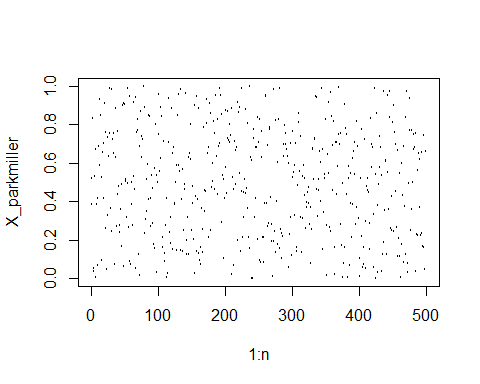
\includegraphics{lesson1_files/figure-latex/unnamed-chunk-3-1.pdf}

\begin{Shaded}
\begin{Highlighting}[]
\NormalTok{sorted\_parkmiller\_X }\OtherTok{\textless{}{-}} \FunctionTok{sort}\NormalTok{(X\_parkmiller)}

\FunctionTok{plot}\NormalTok{(sorted\_parkmiller\_X,(}\DecValTok{1}\SpecialCharTok{:}\NormalTok{n)}\SpecialCharTok{/}\NormalTok{n, }\AttributeTok{type=}\StringTok{\textquotesingle{}s\textquotesingle{}}\NormalTok{, }\AttributeTok{xlim=}\FunctionTok{c}\NormalTok{(}\DecValTok{0}\NormalTok{,}\DecValTok{1}\NormalTok{), }\AttributeTok{ylim=}\FunctionTok{c}\NormalTok{(}\DecValTok{0}\NormalTok{,}\DecValTok{1}\NormalTok{))}
\FunctionTok{abline}\NormalTok{(}\AttributeTok{a=}\DecValTok{0}\NormalTok{,}\AttributeTok{b=}\DecValTok{1}\NormalTok{,}\AttributeTok{col=}\StringTok{"red"}\NormalTok{)}
\end{Highlighting}
\end{Shaded}

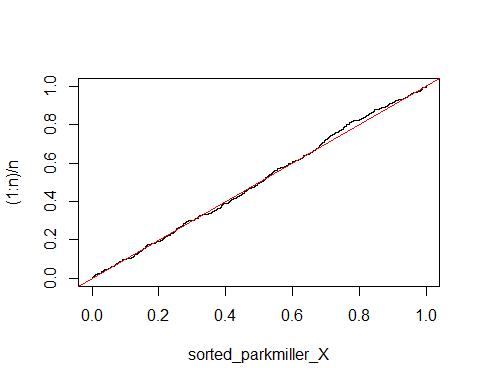
\includegraphics{lesson1_files/figure-latex/unnamed-chunk-3-2.pdf}

\begin{Shaded}
\begin{Highlighting}[]
\NormalTok{x1}\OtherTok{\textless{}{-}}\NormalTok{sorted\_parkmiller\_X[}\DecValTok{1}\SpecialCharTok{:}\NormalTok{(n}\DecValTok{{-}2}\NormalTok{)]}
\NormalTok{x2}\OtherTok{\textless{}{-}}\NormalTok{sorted\_parkmiller\_X[}\DecValTok{2}\SpecialCharTok{:}\NormalTok{(n}\DecValTok{{-}1}\NormalTok{)]}
\NormalTok{x3}\OtherTok{\textless{}{-}}\NormalTok{sorted\_parkmiller\_X[}\DecValTok{3}\SpecialCharTok{:}\NormalTok{n]}
\FunctionTok{library}\NormalTok{(rgl)}
\end{Highlighting}
\end{Shaded}

\begin{verbatim}
## Warning in rgl.init(initValue, onlyNULL): RGL: unable to open X11 display
\end{verbatim}

\begin{verbatim}
## Warning: 'rgl.init' failed, running with 'rgl.useNULL = TRUE'.
\end{verbatim}

\begin{Shaded}
\begin{Highlighting}[]
\FunctionTok{plot3d}\NormalTok{(x1,x2,x3)}
\FunctionTok{plot}\NormalTok{(x1,x3,}\AttributeTok{cex=}\FloatTok{0.5}\NormalTok{)}
\end{Highlighting}
\end{Shaded}

\includegraphics{lesson1_files/figure-latex/unnamed-chunk-3-3.pdf}

\end{document}
